% !TEX TS-program = pdflatex
\documentclass[aspectratio=169]{beamer}
\usepackage[utf8]{inputenc}
\usepackage[T1]{fontenc}
\usetheme{Madrid}
\usecolortheme{seahorse}
\usefonttheme{professionalfonts}
\setbeamertemplate{navigation symbols}{}
\setbeamercovered{transparent}
\setbeamertemplate{itemize items}[circle]
\setbeamertemplate{enumerate items}[default]
\setlength{\parskip}{0.15em}

\definecolor{bepurple}{RGB}{107,63,160}
\definecolor{begold}{RGB}{200,168,75}
\definecolor{beteal}{RGB}{26,122,110}
\definecolor{berust}{RGB}{192,68,42}
\definecolor{beblue}{RGB}{26,74,138}
\definecolor{softpurple}{RGB}{240,232,255}
\definecolor{softgold}{RGB}{255,248,220}
\definecolor{softteal}{RGB}{220,242,240}
\definecolor{softrust}{RGB}{255,235,230}
\setbeamercolor{structure}{fg=beblue}
\setbeamercolor{title}{fg=white,bg=beblue}
\setbeamercolor{frametitle}{fg=beblue}
% Minimal block rendering: regular/example blocks become colored headings (no box)
\setbeamertemplate{block begin}{%
  \par\vspace{0.2ex}%
  \ifx\insertblocktitle\empty\else%
    {\usebeamerfont{block title}\color{beblue}\textbf{\insertblocktitle}}\par\vspace{0.2ex}%
  \fi%
}
\setbeamertemplate{block end}{\par\vspace{0.2ex}}
\setbeamertemplate{block example begin}{%
  \par\vspace{0.2ex}%
  \ifx\insertblocktitle\empty\else%
    {\usebeamerfont{block title}\color{beteal}\textbf{\insertblocktitle}}\par\vspace{0.2ex}%
  \fi%
}
\setbeamertemplate{block example end}{\par\vspace{0.2ex}}
\setbeamertemplate{block alerted begin}{%
  \par\vspace{0.5ex}%
  \begin{beamercolorbox}[sep=0.5ex,rounded=true,shadow=false]{block title alerted}%
    \usebeamerfont{block title}\insertblocktitle%
  \end{beamercolorbox}%
  \nointerlineskip%
  \begin{beamercolorbox}[sep=0.5ex,rounded=true,shadow=false]{block body alerted}%
    \usebeamerfont{block body}%
}
\setbeamertemplate{block alerted end}{\end{beamercolorbox}\par\vspace{0.5ex}}
\setbeamercolor{block title alerted}{fg=white,bg=berust}
\setbeamercolor{block body alerted}{fg=black,bg=berust!8}
\setbeamercolor{alerted text}{fg=berust}

\usepackage{booktabs,amsmath,amssymb,array,multirow,hyperref,colortbl,xcolor}
\usepackage{tikz}
\usepackage{pgfplots}
\pgfplotsset{compat=1.18}
\usetikzlibrary{arrows.meta,positioning,calc,shapes.geometric,patterns}
\hypersetup{colorlinks=true,linkcolor=beblue,urlcolor=beblue}

\title{\textbf{Lecture 4: Time Inconsistency \& Present Bias}}
\subtitle{Why We Make Promises We Cannot Keep}
\author{Prof.\ Muhebullah Karimzada}
\institute{School of Economics, University of Northern British Columbia}
\date{ECON 230 $\cdot$ Introduction to Behavioural Economics $\cdot$ Winter 2027}

\begin{document}

\begin{frame}[plain]\titlepage\end{frame}

% ============================================================
\begin{frame}{The New Year's Resolution Problem}
\note{Start with the relatable. 80\% of New Year's resolutions fail by February. This is not weakness of character -- it is a predictable consequence of how we discount time.}
\begin{columns}
\column{0.5\textwidth}
\begin{alertblock}{The Statistics}
\begin{itemize}\small\setlength{\itemsep}{0pt}
  \item \textbf{80\%} of New Year's resolutions fail by February (Statista, 2023).
  \item \textbf{50\%} of gym memberships purchased in January are unused by March.
  \item \textbf{47\%} of Canadians who intend to start saving ``this year'' have not started by December (FP Canada, 2023).
\end{itemize}
\end{alertblock}
\begin{block}{The Question}
Is this a character defect? Lack of willpower? \textit{Or} is it a predictable feature of how we discount time? \textcolor{bepurple}{\textbf{Today we show it is the latter.}}
\end{block}
\column{0.47\textwidth}
\begin{tikzpicture}
\begin{axis}[
  width=\textwidth,height=0.53\textheight,
  xlabel={\small Week},ylabel={\small \% Still Keeping Resolution},
  xmin=0,xmax=12,ymin=0,ymax=105,
  axis lines=left,
  title={\small Resolution Survival Rate (2023)}
]
\addplot[berust,very thick] coordinates{(0,100)(1,92)(2,81)(3,72)(4,65)(6,55)(8,47)(10,38)(12,31)};
\draw[dashed,beteal] (axis cs:0,80) -- (axis cs:12,80) node[right,font=\tiny,beteal]{};
\node[font=\tiny,berust] at (axis cs:10,25){\textbf{Only 31\% survive}};
\end{axis}
\end{tikzpicture}
\end{columns}
\end{frame}

% ============================================================
\begin{frame}{Lecture Roadmap}
\begin{enumerate}[<+->]
  \item \textbf{Exponential discounting} --- the standard model and its properties
  \item \textbf{Evidence that exponential discounting fails} --- declining discount rates
  \item \textbf{Hyperbolic discounting} --- the alternative
  \item \textbf{The $\beta$-$\delta$ model} --- quasi-hyperbolic discounting
  \item \textbf{Procrastination} --- why we delay even when we shouldn't
  \item \textbf{Naivety vs sophistication} --- do we know we'll procrastinate?
  \item \textbf{Commitment devices} --- solutions for sophisticated agents
  \item \textbf{Applications:} savings, addiction, smoking, gambling
  \item \textbf{Policy implications:} sin taxes, defaults, mandatory savings
\end{enumerate}
\end{frame}

% ============================================================
\section{Standard Discounting}
% ============================================================

\begin{frame}{Exponential Discounting --- The Standard Model}
\begin{block}{The Model}
A rational agent with discount factor $\delta \in (0,1)$ values future utility as:
\[
  U_t = \sum_{\tau=0}^{\infty} \delta^\tau \, u(c_{t+\tau})
\]
Each period discounted at a \textbf{constant} rate: $r = 1/\delta - 1$.
\end{block}
\begin{columns}
\column{0.5\textwidth}
\begin{block}{Three Reasons to Discount}
\begin{enumerate}
  \item \textbf{Opportunity cost:} \$100 today can earn interest.
  \item \textbf{Uncertainty:} The future may not arrive.
  \item \textbf{Pure time preference:} Impatience for its own sake.
\end{enumerate}
\end{block}
\column{0.47\textwidth}
\begin{block}{Key Property: Time Consistency}
If on \textbf{Monday} you prefer \$110 on Friday over \$100 on Thursday, then on \textbf{Thursday} you should \textit{still} prefer \$110 tomorrow over \$100 today. The ranking of future options \textbf{does not change} as they approach. ``Self$_0$ and Self$_t$ always agree.''
\end{block}
\end{columns}
\end{frame}

% ============================================================
\begin{frame}{Thaler's Evidence --- Declining Discount Rates}
\begin{block}{Thaler (1981) --- Experimental Method}
Participants asked: ``What amount of money in the future would make you indifferent to receiving \$15 today?''
\end{block}
\medskip
\begin{center}
\begin{tabular}{lccc}
\toprule
\textbf{Amount now} & \textbf{Delay: 1 month} & \textbf{Delay: 1 year} & \textbf{Delay: 10 years}\\
\midrule
\$15 now $\to$ \$X later & Median: \$20 & Median: \$50 & Median: \$100\\[0.3em]
\textit{Implied annual rate} & \textit{345\%} & \textit{120\%} & \textit{19\%}\\
\bottomrule
\end{tabular}
\end{center}
\medskip
\begin{alertblock}{The Violation of Exponential Discounting}
Exponential discounting predicts a \textbf{constant} annual discount rate regardless of horizon. But the data show rates \textit{falling sharply} from 345\% (short horizon) to 19\% (long horizon). This \alert{``decreasing impatience''} cannot be explained by any constant-rate model.
\end{alertblock}
\end{frame}

% ============================================================
\begin{frame}{Declining Discount Rates --- The Evidence Graphically}
\begin{center}
\begin{tikzpicture}
\begin{axis}[
  width=0.80\textwidth,height=0.55\textheight,
  xlabel={Delay (months)},ylabel={Implied Annual Rate (\%)},
  xmin=0,xmax=125,ymin=0,ymax=400,
  axis lines=left,
  title={Thaler (1981): Observed vs Predicted Discount Rates},
  xtick={1,12,120},xticklabels={1 month,1 year,10 years}
]
\addplot[berust,very thick,mark=*,mark size=3pt] coordinates{(1,345)(12,120)(120,19)};
\addplot[beteal,dashed,thick,domain=0:120]{60};
\node[font=\small,beteal] at (axis cs:88,70) {Exponential (constant)};
\node[font=\small,berust] at (axis cs:25,310) {Observed (declining)};
\end{axis}
\end{tikzpicture}
\end{center}
\begin{exampleblock}{Key Insight}
The steep drop in the short run (345\% $\to$ 120\%) followed by a flat tail is the signature of \alert{hyperbolic discounting} --- the model we study next.
\end{exampleblock}
\end{frame}

% ============================================================
\section{Hyperbolic Discounting}
% ============================================================

\begin{frame}{Hyperbolic Discounting}
Instead of $\delta^t$ (constant decay), use: $D(t) = \dfrac{1}{1 + \alpha t}$. This generates a \alert{discount rate that falls over time} --- matching the empirical evidence.
\begin{columns}
\column{0.5\textwidth}
\begin{tikzpicture}
\begin{axis}[
  width=\textwidth,height=0.60\textheight,
  xlabel={\small Time Period},ylabel={\small Discount Factor},
  xmin=0,xmax=20,ymin=0,ymax=1.05,
  axis lines=left,
  title={\small Exponential vs Hyperbolic},
  legend pos=north east
]
\addplot[beteal,very thick,domain=0:20,samples=50]{0.9^x};
\addplot[berust,very thick,domain=0:20,samples=100]{1/(1+0.5*x)};
\legend{\small Exponential ($\delta=0.9$),\small Hyperbolic ($\alpha=0.5$)}
\end{axis}
\end{tikzpicture}
\column{0.47\textwidth}
\begin{alertblock}{The Key Difference}
\textbf{Steep initial drop:} present overweighted vs near future. \textbf{Flat tail:} future periods roughly equally valued. This initial drop \textit{is} present bias.
\end{alertblock}
\textcolor{beteal}{\textbf{Dynamic Inconsistency:}} Preferences \textbf{reverse} as time passes --- you prefer to exercise tomorrow over today, but tomorrow you prefer the day after. Ad infinitum.
\end{columns}
\end{frame}

% ============================================================
\begin{frame}{The $\beta$-$\delta$ Model (Quasi-Hyperbolic)}
\[
  U_t = u(c_t) + \beta \sum_{\tau=1}^{\infty} \delta^\tau \, u(c_{t+\tau})
\]
$\beta \in (0,1)$: \alert{present bias} (extra future discounting). $\delta$: long-run patience. $\beta=1$: reduces to exponential.
\begin{columns}
\column{0.5\textwidth}
\textcolor{beblue}{\textbf{Calibrated Parameters:}} $\beta \approx 0.7$--$0.8$; $\delta \approx 0.95$--$0.99$.

$\beta = 0.7$: tomorrow is worth only \textbf{70\%} as much as today, \textit{regardless of how far away tomorrow is}.
\column{0.47\textwidth}
\begin{tikzpicture}
\begin{axis}[
  width=\textwidth,height=0.55\textheight,
  xlabel={\small Period},ylabel={\small Discount Weight},
  xmin=0,xmax=8,ymin=0,ymax=1.05,
  axis lines=left,
  title={\small $\beta$-$\delta$ vs Exponential ($\beta=0.7$, $\delta=0.97$)},
  legend pos=north east
]
\addplot[beteal,thick,mark=square*,mark size=2pt] coordinates{(0,1)(1,0.97)(2,0.9409)(3,0.9127)(4,0.8853)(5,0.8587)(6,0.8330)(7,0.8080)};
\addplot[berust,thick,mark=*,mark size=2pt] coordinates{(0,1)(1,0.7)(2,0.679)(3,0.659)(4,0.639)(5,0.620)(6,0.601)(7,0.583)};
\draw[<->,thin,bepurple,thick] (axis cs:1,0.97) -- (axis cs:1,0.70)
  node[midway,right,font=\tiny,bepurple,align=left]{$\beta = 0.7$\\(present\\bias drop)};
\legend{\small Exponential ($\delta=0.97$),\small $\beta$-$\delta$ ($\beta=0.7$, $\delta=0.97$)}
\end{axis}
\end{tikzpicture}
\end{columns}
\end{frame}

% ============================================================
\section{Procrastination}
% ============================================================

\begin{frame}{Why We Procrastinate}
\begin{block}{O'Donoghue \& Rabin (1999, 2001)}
A present-biased agent faces a task: cost $c$ today, benefit $b$ in the future. The agent does the task \textit{today} if:
\[
  u_{\text{today}}(\text{do}) \geq u_{\text{today}}(\text{wait})
\]
With present bias: doing today has cost $c$ (no discounting), benefit $b$ discounted by $\beta$. Waiting has cost $c$ discounted by $\beta$ (since it's in the future). When $b$ is far in the future, the agent keeps preferring to wait --- every day.
\end{block}
\begin{exampleblock}{The Procrastination Trap}
\textbf{Monday:} ``I'll clean my room on Saturday'' (Saturday cost is discounted by $\beta$).\\
\textbf{Saturday morning:} ``I'll clean tomorrow'' (tomorrow's cost is again discounted by $\beta$).\\
\textbf{Same logic applies every period.} The agent never cleans.
\end{exampleblock}
\end{frame}

% ============================================================
\begin{frame}{[GAME] The Homework Problem}
\note{This is a reveal game. First ask about intention (raise hands). Then ask about actual behaviour (how many did last assignment the night before). The gap between stated preference and actual behaviour is present bias.}
\begin{alertblock}{Scenario}
You have a take-home essay due at the \textbf{end of term} (6 weeks away). You can write it any time. It takes 3 hours.\\[0.4em]
The benefit (grade) arrives at end of term regardless of when you write it.\\[0.4em]
\textbf{Poll:} When do you plan to write it?\\[0.2em]
\quad A) This week \quad B) In 2--3 weeks \quad C) The week before \quad D) The night before
\end{alertblock}
\pause
\begin{block}{Second Poll}
\textbf{Honestly:} How many of you did your most recent assignment \textit{earlier than 48 hours before the deadline}?
\end{block}
\pause
\begin{exampleblock}{The Gap}
The gap between \textit{intended} timing (this week) and \textit{actual} timing (night before) is exactly what the $\beta$-$\delta$ model predicts. This gap is \alert{present bias in action}.
\end{exampleblock}
\end{frame}

% ============================================================
\begin{frame}{Naivety vs Sophistication}
\begin{block}{O'Donoghue \& Rabin (2001)}
Present-biased agents can differ in their \textit{self-knowledge}:
\end{block}
\begin{columns}
\column{0.5\textwidth}
\begin{block}{\textcolor{berust}{Naïve Agent} ($\hat{\beta} = 1$)}
Does \textbf{not know} they are present-biased. Believes their future self will follow through on plans. Perpetually surprised by their own failure to act.\\[0.3em]
\textit{``I'll definitely start my diet next Monday.''} (Said every Monday for a year.)\\[0.3em]
Does not use commitment devices --- sees no need.
\end{block}
\column{0.47\textwidth}
\begin{block}{\textcolor{beteal}{Sophisticated Agent} ($\hat{\beta} = \beta$)}
\textbf{Knows} they are present-biased. Anticipates future self-control failures. May use commitment devices NOW to constrain the future self.\\[0.3em]
\textit{Ulysses and the Sirens}: tied himself to the mast before hearing the sirens.\\[0.3em]
\textit{Ariely \& Wertenbroch (2002)}: students chose self-imposed deadlines for papers --- and performed better.
\end{block}
\end{columns}
\end{frame}

% ============================================================
\begin{frame}{Evidence on Procrastination}
\textcolor{beblue}{\textbf{Ariely \& Wertenbroch (2002):}} Three MIT paper configurations:
\begin{enumerate}\small
  \item \textbf{Imposed evenly spaced:} best grades.
  \item \textbf{Self-imposed evenly spaced:} second best.
  \item \textbf{All at end:} worst grades.
\end{enumerate}
\begin{columns}
\column{0.5\textwidth}
\begin{alertblock}{Lesson 1: Deadlines Work}
Self-imposed deadlines improve performance. Present-biased agents benefit from commitment to milestones.
\end{alertblock}
\column{0.47\textwidth}
\begin{alertblock}{Lesson 2: Partial Sophistication}
Students \textit{chose} to space deadlines, showing awareness of procrastination --- but many clustered too tightly at the end.
\end{alertblock}
\end{columns}
\textcolor{beteal}{\textbf{UBC (2019):}} Digital calendar reminders $\Rightarrow$ +0.4 GPA points vs controls. Technology as a commitment device.
\end{frame}

% ============================================================
\section{Savings and Commitment}
% ============================================================

\begin{frame}{The Undersaving Puzzle --- Canadian Data}
\begin{columns}
\column{0.5\textwidth}
\textcolor{beblue}{\textbf{Savings Rate (Statistics Canada):}}
\begin{itemize}\small
  \item 1982: \textbf{20.2\%} $\to$ 2005: \textbf{2.5\%} (historic low)
  \item 2020--21: \textbf{12--28\%} (COVID) $\to$ 2024: \textbf{$\approx$5.3\%}
\end{itemize}
\begin{alertblock}{The RRSP Gap}
\begin{itemize}\small
  \item Only \textbf{27\%} contributed (2022); unused room: \$25K+.
  \item \textbf{41\%} have \textit{no} retirement savings (BMO, 2023).
  \item 93\% \textit{know} RRSPs exist. The problem is present bias.
\end{itemize}
\end{alertblock}
\column{0.47\textwidth}
\begin{tikzpicture}
\begin{axis}[
  width=\textwidth,height=0.60\textheight,
  xlabel={\small Year},ylabel={\small Savings Rate (\%)},
  xmin=1980,xmax=2025,ymin=0,ymax=32,
  axis lines=left,
  title={\small Canadian Household Savings Rate}
]
\addplot[beblue,very thick] coordinates{
  (1982,20.2)(1985,17)(1990,13)(1995,9)(2000,5.3)(2005,2.5)
  (2008,5)(2010,6)(2015,4)(2019,3.5)(2020,12)(2021,28)(2022,7)(2024,5.3)
};
\draw[dashed,beteal] (axis cs:1980,10) -- (axis cs:2025,10) node[right,font=\tiny,beteal]{10\% target};
\end{axis}
\end{tikzpicture}
\end{columns}
\end{frame}

% ============================================================
\begin{frame}{SAVE MORE TOMORROW (SMarT)}
\textcolor{beblue}{\textbf{Thaler \& Benartzi (2004):}} Commit TODAY to save more starting with your \textbf{next pay raise}: (1) commitment before temptation; (2) raise offsets loss aversion; (3) automatic.
\begin{columns}
\column{0.5\textwidth}
\begin{tikzpicture}
\begin{axis}[
  width=\textwidth,height=0.58\textheight,
  ybar,bar width=0.55cm,
  ylabel={\small Savings Rate (\%)},
  symbolic x coords={Baseline,Year 1,Year 2,Year 3},
  xtick=data,ymin=0,ymax=14,
  nodes near coords,
  title={\small SMarT Program Results}
]
\addplot[fill=beteal!70] coordinates{(Baseline,3.5)(Year 1,6.5)(Year 2,9.4)(Year 3,11.6)};
\addplot[fill=berust!50] coordinates{(Baseline,3.5)(Year 1,3.6)(Year 2,3.7)(Year 3,3.8)};
\legend{\small SMarT group,\small Control group}
\end{axis}
\end{tikzpicture}
\column{0.47\textwidth}
\begin{exampleblock}{The Results}
\begin{itemize}
  \item Savings rate: $3.5\% \to 11.6\%$ in 3 years.
  \item Participation: $3.5\% \to 13.6\%$.
  \item Control group: essentially unchanged.
  \item US Pension Protection Act (2006) institutionalised this nationwide.
  \item \textbf{British Columbia} WorkSafeBC pension: automatic escalation adopted 2018.
\end{itemize}
\end{exampleblock}
\end{columns}
\end{frame}

% ============================================================
\begin{frame}{Commitment Devices}
\begin{block}{Definition}
A \alert{commitment device} is a mechanism that a sophisticated present-biased agent uses \textit{now} to constrain their future self. It makes the future temptation either unavailable or costly.
\end{block}
\begin{columns}
\column{0.5\textwidth}
\begin{exampleblock}{Historical Examples}
\begin{itemize}
  \item \textbf{Ulysses and the Sirens:} tied to the mast before the temptation arrived.
  \item \textbf{Christmas clubs:} low-interest savings accounts locked until December.
  \item \textbf{Layaway plans:} commit to purchase via installments.
  \item \textbf{SEED accounts (Philippines):} Ashraf, Karlan \& Yin (2006) --- savings 82\% higher than control after 12 months.
\end{itemize}
\end{exampleblock}
\column{0.47\textwidth}
\begin{exampleblock}{Modern Examples}
\begin{itemize}
  \item \textbf{stickK.com}: pledge money against a goal. If you fail, the money goes to a charity you hate. $\approx\$700$K/day in active stakes.
  \item \textbf{Automatic savings transfers:} Simplii Financial (Canada), Chime.
  \item \textbf{Gym contracts:} pre-pay for a year to make yourself go.
  \item \textbf{Smoking bans} at home: remove availability.
\end{itemize}
\end{exampleblock}
\end{columns}
\end{frame}

% ============================================================
\begin{frame}{[GAME] Design a Commitment Device}
\note{Group activity. Give 4 minutes. Each group presents their best commitment device. Evaluate: Does it work for a naive agent? A sophisticated agent? Can future-self circumvent it?}
\begin{alertblock}{Group Exercise --- 4 Minutes}
Your friend says: ``I know I should exercise 3 times a week, but I keep skipping the gym when I'm tired. I've been saying this for 6 months.''
\medskip

\textbf{Design a commitment device} that:
\begin{enumerate}
  \item Works even when your friend is tired and unmotivated.
  \item Does not require strong willpower in the moment.
  \item Your friend cannot easily circumvent.
\end{enumerate}
\end{alertblock}
\begin{block}{Evaluation Criteria}
\begin{itemize}
  \item Does it address \textit{when} costs and benefits occur?
  \item Does it involve a \textit{pre-commitment} before the temptation?
  \item Is it \textit{credibly binding}? Can future-self escape?
\end{itemize}
\end{block}
\end{frame}

% ============================================================
\section{Addiction \& Policy}
% ============================================================

\begin{frame}{Present Bias and Addiction}
Addictive goods: immediate payoff + delayed cost. Present bias ($\beta < 1$) causes systematic \textit{over-consumption} because future costs are heavily discounted.
\begin{exampleblock}{Canadian Smoking Data}
\begin{itemize}\small
  \item 13\% smoke (2019) --- down from 50\% in 1966.
  \item 70\% \textit{want} to quit; 50\% try/year; only \textbf{5\%} succeed without aids.
  \item ``I'll quit Monday'' --- said every week, for years. Classic naive present bias.
  \item BC ``QuitNow'': 23\% 6-month quit rate vs 5\% unassisted.
\end{itemize}
\end{exampleblock}
\begin{alertblock}{Policy: Corrective Taxes}
O'Donoghue \& Rabin (2006): if $\beta < 1$ and agents are \textit{naive}, a Pigouvian tax is optimal even with \textit{perfect information} --- over-consumption relative to own long-run preferences.
\end{alertblock}
\end{frame}

% ============================================================
\begin{frame}{Discussion Questions}
\begin{enumerate}
  \item[\textcolor{bepurple}{Q1.}] ``Are you a sophisticated or na\"{i}ve present-biased agent? How do you know? Can you think of a commitment device you've successfully used?''
  \medskip
  \item[\textcolor{beteal}{Q2.}] ``Is it paternalistic for the government to require mandatory retirement savings (like Australia's Superannuation at 11\%)? Or is it correcting a cognitive bias that people themselves want to correct?''
  \medskip
  \item[\textcolor{berust}{Q3.}] ``Should cigarette taxes be \textit{higher} if people are na\"{i}vely present-biased? How does your answer change if people are \textit{sophisticated}?''
\end{enumerate}
\end{frame}

% ============================================================
\begin{frame}{Key Takeaways --- Lecture 4}
\begin{itemize}
  \item[\textcolor{beteal}{\checkmark}] \textbf{Exponential discounting:} constant rate, time consistent --- self$_0$ and self$_t$ always agree.
  \item[\textcolor{beteal}{\checkmark}] \textbf{Evidence:} discount rates decline with horizon --- violates exponential model.
  \item[\textcolor{beteal}{\checkmark}] \textbf{Hyperbolic discounting:} steep initial drop + flat tail = present bias.
  \item[\textcolor{beteal}{\checkmark}] \textbf{$\beta$-$\delta$ model:} $\beta < 1$ = present bias; $\delta$ = long-run patience.
  \item[\textcolor{beteal}{\checkmark}] \textbf{Time inconsistency:} choices reverse as future becomes present. Preferences flip.
  \item[\textcolor{beteal}{\checkmark}] \textbf{Na\"{i}ve vs sophisticated:} na\"{i}ves cycle through failed resolutions; sophisticates pre-commit.
  \item[\textcolor{beteal}{\checkmark}] \textbf{Commitment devices:} work by constraining future self before temptation arrives.
  \item[\textcolor{beteal}{\checkmark}] \textbf{Applications:} procrastination, undersaving, addiction, SMarT program.
\end{itemize}
\medskip\textcolor{beblue}{\textbf{Next:}} \textbf{Lecture 5: Intertemporal Choice \& Savings} --- Mental accounting, why we hold debt and savings simultaneously, and the Canadian retirement savings crisis.
\end{frame}

% ============================================================
\begin{frame}{Further Reading}
\begin{itemize}
  \item Laibson, D.\ (1997). Golden eggs and hyperbolic discounting. \textit{QJE}, 112(2), 443--477.
  \item O'Donoghue, T.\ \& Rabin, M.\ (1999). Doing it now or later. \textit{AER}, 89(1), 103--124.
  \item Thaler, R.H.\ \& Benartzi, S.\ (2004). Save more tomorrow. \textit{JPE}, 112(S1), S164--S187.
  \item Ariely, D.\ \& Wertenbroch, K.\ (2002). Procrastination, deadlines, and performance. \textit{Psychological Science}, 13(3), 219--224.
  \item Ashraf, N., Karlan, D.\ \& Yin, W.\ (2006). Tying Odysseus to the mast. \textit{QJE}, 121(2), 635--672.
\end{itemize}
\end{frame}

\end{document}
